
\documentclass[10pt,a4paper,twocolumn]{article}
\usepackage[a4paper,top=1.25cm,bottom=1.45cm,left=1.35cm,right=1.35cm,columnsep=0.55cm]{geometry}
\usepackage{libertinus}
\usepackage{microtype}
\usepackage{graphicx,booktabs,tabularx,array,multirow}
\usepackage[dvipsnames]{xcolor}
\usepackage{enumitem}
\usepackage{titlesec}
\usepackage[skins]{tcolorbox}
\usepackage[font=footnotesize,labelfont={bf,sf},labelsep=period,skip=3pt]{caption}
\usepackage[colorlinks=true,urlcolor=accent,linkcolor=accent]{hyperref}
\definecolor{navy}{HTML}{1D2B4F}
\definecolor{accent}{HTML}{B42318}
\definecolor{muted}{HTML}{6B7280}
\definecolor{boxbg}{HTML}{F4F6FB}
\titleformat{\section}{\sffamily\bfseries\large\color{navy}}{\thesection}{0.5em}{}[\vspace{-0.55em}\textcolor{navy}{\rule{\columnwidth}{0.6pt}}]
\titleformat{\subsection}{\sffamily\bfseries\normalsize\color{navy}}{\thesubsection}{0.5em}{}
\titlespacing*{\section}{0pt}{7pt}{3pt}
\titlespacing*{\subsection}{0pt}{5pt}{2pt}
\setlist{nosep,leftmargin=1.1em,itemsep=1.6pt}
\setlength{\parskip}{2pt}\setlength{\parindent}{0pt}
\setlength{\textfloatsep}{7pt}\setlength{\floatsep}{6pt}\setlength{\dbltextfloatsep}{7pt}\setlength{\abovecaptionskip}{2pt}
\newcommand{\obs}[1]{\textbf{\color{navy}#1}\ }
\pagestyle{plain}

\begin{document}
\twocolumn[{%
\begin{center}
{\sffamily\bfseries\LARGE\color{navy} How three CSIR chemistry laboratories publish, connect\\[2pt] and measure up to the world, 2016--2026\par}
\vspace{5pt}
{\sffamily\normalsize \textbf{Group 24}\quad$\cdot$\quad Samarth Singla $\cdot$ Sanjith Ganapathi $\cdot$ Prathmesh Sharma\par}
\vspace{2pt}
{\sffamily\small CSIR-NCL (Pune) $\cdot$ CSIR-IICT (Hyderabad) $\cdot$ CSIR-CECRI (Karaikudi) $\cdot$ DPCN 2026\par}
\vspace{2pt}
{\sffamily\small Interactive dashboard: \href{https://dpcnsite.vercel.app/}{\textbf{https://dpcnsite.vercel.app/}}\par}
\end{center}
\vspace{2pt}
\begin{tcolorbox}[enhanced,colback=boxbg,colframe=navy!55,boxrule=0.6pt,arc=1.5pt,left=6pt,right=6pt,top=4pt,bottom=4pt]
{\sffamily\bfseries\color{navy} Key observations}\\[1pt]
\small
\begin{tabularx}{\linewidth}{@{}>{\bfseries\color{accent}}l@{\hspace{6pt}}X@{}}
1 & \textbf{Output is shrinking, and the decline is real.} 1,727 papers in 2016, 1,208 in 2025 (-3.9\% a year), driven by IICT (-4.9\%) and NCL (-4.3\%); NCL's own annual report confirms the scale. \\
2 & \textbf{Fewer papers, but a larger share in top journals.} Q1 papers in journals with IF\,$>$\,5 rose from 17.0\% to 39.4\% of output (IF\,$>$\,10: 1.8\% $\to$ 8.5\%). CECRI, the smallest lab, leads on every quality measure. \\
3 & \textbf{Three islands.} Only 0.8\% of co-authorship links join two labs, yet 19.7\% of citations between scientists do: the labs read each other but rarely write together. \\
4 & \textbf{Against their closest foreign counterparts the labs trail most at the top.} Compared with nine ``twin'' institutes chosen by fixed rules in the USA, China, South Korea and Australia, the labs' median share of papers in the world's top 10\% is 2.0$\times$ lower, and their share in Q1 journals with IF\,$>$\,10 is 3.1$\times$ lower; the gap grows as the bar rises. \\
5 & \textbf{Knowledge flows in from abroad by reading, and out to Indian universities.} The labs cite 4,461 papers of their foreign peers but co-authored 49 with them; Indian universities draw on the labs' work more than the reverse (1.63--2.00$\times$). In the labs' own citations, ideas pass over a co-authorship tie only 0.81\% of the time, below the tipping point of 6\%. \\
\end{tabularx}
\end{tcolorbox}
\vspace{4pt}
}]

\section{Data and approach}
Every peer-reviewed paper (2016--2026) with an author at one of the three laboratories was collected from OpenAlex, with each laboratory resolved to its ROR and OpenAlex identifiers and mis-tagged papers recovered from raw affiliation strings. The corpus has 14,208 distinct papers (14,029 journal, 179 conference) by 7,820 lab authors; \textbf{faculty} are the 306 scientists on the institutes' staff pages (382 after cleaning) with at least one paper. Quartiles are SCImago's best quartile in the publication year; as \textbf{impact factor (IF)} we use SCImago's two-year citations per document in the same year, a Scopus analogue of the JIF, known for 94.2\% of papers. The scale was checked against an independent source: NCL's annual report lists 467, 407 and 365 papers for 2021--2023; our data has 461, 415, 417.

\section{Basic statistics}
\begin{table*}[t]
\centering\small
\caption{Overview, 2016--2026 (distinct papers; a paper shared by two labs counts for each, once in ``All three''). Percentages of all papers. Growth = compound yearly change 2016$\to$2025 (2026 is a partial year). Citations: OpenAlex counts, not field-normalised. h-index: 2016--2026 papers, roster scientists.}
\begin{tabular}{@{}lrrrrrrrrrr@{}}
\toprule
Lab & Papers & Q1 (\%) & Q1\,\&\,IF$>$5 & Q1\,\&\,IF$>$10 & $<$10 authors & Mean & Intl. & Citations & h-index & Growth \\
 & & & (\%) & (\%) & (\%) & authors & (\%) & mean\,/\,median & mean\,/\,max & (\%/yr) \\
\midrule
NCL & 5,316 & 64.2 & 29.3 & 7.3 & 93.5 & 5.2 & 18.2 & 25.2\,/\,11 & 10.1\,/\,43 & -4.3 \\
IICT & 6,123 & 51.2 & 23.6 & 3.7 & 93.8 & 5.5 & 22.1 & 20.4\,/\,10 & 8.6\,/\,54 & -4.9 \\
CECRI & 2,870 & 70.0 & 39.8 & 7.2 & 95.3 & 5.2 & 30.4 & 32.4\,/\,17 & 14.0\,/\,59 & +0.1 \\
\textbf{All three} & \textbf{14,208} & \textbf{59.7} & \textbf{28.8} & \textbf{5.7} & \textbf{94.1} & \textbf{5.3} & \textbf{22.3} & \textbf{24.6\,/\,11} & \textbf{9.8\,/\,59} & \textbf{-3.9} \\
\bottomrule
\end{tabular}
\end{table*}

\begin{figure*}[t]
\centering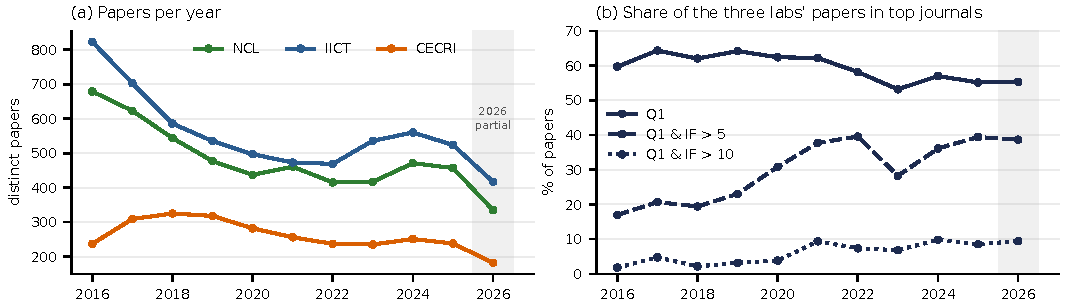
\includegraphics[width=\textwidth]{fig_trends.pdf}
\caption{(a) Papers per year per lab; 2026 (shaded) runs to the collection date in October. (b) Share of the three labs' papers in Q1 journals, in Q1 journals with IF\,$>$\,5 and with IF\,$>$\,10.}
\end{figure*}

\obs{Output is falling, and the fall is real.} The labs published 1,727 papers in 2016 and 1,208 in 2025 (-3.9\% a year). IICT (-4.9\%) and NCL (-4.3\%) drive the decline; CECRI is flat (+0.1\%). The steepest fall was 2016--2020; output has levelled since.

\obs{Quality moved up while volume fell.} 59.7\% of all papers are in Q1 journals, 28.8\% in Q1 journals with IF\,$>$\,5 and 5.7\% with IF\,$>$\,10. Over time the plain Q1 share dipped (59.7\% $\to$ 55.1\%) but the high-IF shares rose sharply (Fig.~1b), so papers moved towards the top of the Q1 band (journal citation rates also drift upwards, so part of this is inflation of IF). By lab, the Q1 share of ranked journal papers fell at IICT (64.7\% $\to$ 46.8\%) and NCL (74.2\% $\to$ 61.3\%) and held at CECRI (79.2\% $\to$ 74.0\%).

\obs{The smallest lab has the highest quality.} CECRI (2,870 papers) leads at every threshold: Q1 70.0\%, Q1\,\&\,IF\,$>$\,5 39.8\%. NCL has the most papers in IF\,$>$\,10 Q1 journals (387); IICT, the largest lab, has about half NCL's share at that level (3.7\% vs 7.3\%).

\obs{Small teams, wide partnerships.} 94.1\% of papers have fewer than 10 authors (mean 5.3, rising from 4.85 to 5.89; only 17 papers have 30 or more): this is small-group bench chemistry. Yet the labs co-author with 3,027 institutions in 95 countries: 22.3\% of papers have a foreign co-author and 45.5\% another Indian institution, and 88.7\% cite and 73.9\% are cited by another Indian institution.

\obs{Journals and fields.} Output is spread thin: no journal carries more than 3.1\% of the papers. The most-used venue is \textit{ChemistrySelect} (Q2) for IICT and \textit{ChemistrySelect} (Q2) for NCL, while CECRI's top two are \textit{Electrochimica Acta} (Q1) and \textit{Journal of Materials Chemistry A} (Q1). By OpenAlex field the cluster is Chemistry 26.9\%, Engineering 19.2\%, Materials Science 18.1\%, Energy 10.5\%; IICT is mainly Chemistry 37.5\%, CECRI Engineering 37.4\%, NCL the broadest (Chemistry 26.8\%).

\obs{Faculty and departments.} 37.6\% of active scientists have an h-index (2016--2026 papers) of 4 or less, and CECRI is bimodal (50\% below 5, 27\% at 25 or more). The highest are Subrata Kundu (CECRI, 59), S. Venkata Mohan (IICT, 54), Sreekumar Kurungot (NCL, 43). The most productive department is Physical and Materials Chemistry Division (NCL; 1,228 papers, 74.3\% Q1, mean h 14.0).

\obs{Citations are concentrated.} 350,015 citations, mean 24.6 but median 11 per paper; the most cited is a review, \textit{Recent Trends and Perspectives in Electrochemical Water Splitt\ldots} (ACS Catalysis, 2016; 2,493 citations). Output is concentrated too: 18 scientists ($\sqrt{N}$) write 36.9\% of faculty papers (Price's law predicts 50\%); Gini 0.61 for papers, 0.73 for citations.

\section{Network analysis}
\begin{table}[t]
\centering\footnotesize\setlength{\tabcolsep}{3.2pt}
\caption{The four networks (2016--2026). $\langle k\rangle$: mean degree (citation: mean in-degree). Cross = share of links joining two labs.}
\begin{tabular}{@{}lrrrrr@{}}
\toprule
Network & Nodes & Links & $\langle k\rangle$ & Comm. ($Q$) & Cross (\%) \\
\midrule
Co-authorship, all lab authors & 7,820 & 35,014 & 8.9 & 136 (0.82) & 0.8 \\
Co-authorship, faculty & 306 & 627 & 4.1 & 12 (0.69) & 2.7 \\
Citation, paper $\to$ paper & 10,931 & 27,099 & 1.9 & -- & 5.9 \\
Citation, scientist $\to$ scientist & 247 & 1,739 & -- & -- & 19.7 \\
\bottomrule
\end{tabular}
\end{table}

\begin{figure}[t]
\centering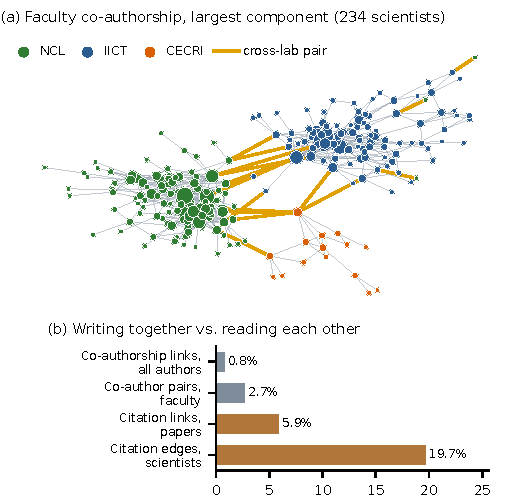
\includegraphics[width=\columnwidth]{fig_network.pdf}
\caption{(a) Faculty co-authorship network; colour = lab, amber = a pair from two labs; size = co-authors. (b) Share of links that cross labs, by network.}
\end{figure}

\obs{One giant component made of tight groups.} 95.8\% of the 7,820 lab authors form one connected component, but the network is sparse (density 0.0011) and highly modular: 136 communities, modularity 0.82. These are research groups: each of the 15 largest is at least 94\% one lab.

\obs{The labs are islands.} Only 0.8\% of co-authorship links and 17 of 627 faculty pairs join two labs; 68 of 306 scientists (22.2\%) have no paper with another roster scientist and connect only through students and project staff.

\obs{They read each other, but do not write together.} 19.7\% of citations between scientists cross labs, 7 times the share of faculty co-author pairs, and half of citing relations are returned (reciprocity 0.51). Between papers, 1,639 of 27,582 citation links (5.9\%) cross labs: IICT$\to$NCL 587, NCL$\to$IICT 404; CECRI sends 322 and receives 326.

\obs{Hubs, not a club.} 93.4\% of researchers have fewer co-authors than their co-authors (mean 9.0 vs 32.1: the friendship paradox), yet the best-connected researchers avoid each other (rich-club coefficient 0.73 of random): each runs a separate group. Removing the 886 best bridges (11.5\%) halves the network; random removal needs 3,325 (Table~\ref{tab:findings}). The top bridges by betweenness are B. Sridhar (IICT), Jagadeesh Babu Nanubolu (IICT), Subrata Kundu (CECRI); the two IICT scientists run X-ray crystallography, a service that appears on many groups' papers. By PageRank, 4 of the 5 most central papers are CECRI's electrocatalysis papers: the smallest lab supplies the most-reused knowledge inside the cluster.

\section{The labs in a global frame}
\textbf{Choosing fair comparators.} We first asked whom the labs actually work with: 22.3\% of papers have a co-author in one of 95 countries, led by the USA (564 papers), South Korea (477) and Australia (408). These three, plus China, the world's largest producer in these subjects (share of world papers 14.0\% $\to$ 31.6\% in 2016--2025) although only the labs' \#5 partner, are the benchmark countries. Everyone is measured on the same \textbf{scope}, the 31 subfields that make up 90\% of the labs' papers, with the same OpenAlex queries (articles and reviews, 2016--2025). In each country a ``twin'' for each lab was selected by fixed rules: the 200 largest institutions in scope; government or facility institutes only, as CSIR labs are (umbrella bodies and 46 hand-reviewed university-hosted labs, consortia and ministries removed, each with a written reason); at least half the size of the smallest lab; and the highest \textbf{cosine similarity} of subfield profiles, one twin per lab, minimum 0.4. Of 800 candidates, 48 reached the similarity test and 9 became twins (Table~\ref{tab:peers}). Six leading Indian institutes (IISc, IIT Bombay, IIT Madras, ICT Mumbai, IACS, IISER Pune) are the home reference.

\begin{table}[t]
\centering\footnotesize\setlength{\tabcolsep}{2.6pt}
\caption{Final peer list: each lab's twin per country with its similarity (1 = identical mix of subfields). ---: no twin; in brackets the most similar institute not already another lab's twin (below 0.4).}\label{tab:peers}
\begin{tabular}{@{}l>{\raggedright}p{1.42cm}>{\raggedright}p{1.42cm}>{\raggedright}p{1.42cm}>{\raggedright\arraybackslash}p{1.42cm}r@{}}
\toprule
Lab & USA & China & S.\ Korea & Australia & Twins \\
\midrule
NCL & ORNL \textcolor{muted}{0.48} & DICP \textcolor{muted}{0.77} & KRICT \textcolor{muted}{0.66} & CSIRO Manuf. \textcolor{muted}{0.70} & 4/4 \\
IICT & --- \textcolor{muted}{(PNNL 0.25)} & SIOC \textcolor{muted}{0.97} & --- \textcolor{muted}{(KBSI 0.38)} & --- \textcolor{muted}{(QIMR 0.09)} & 1/4 \\
CECRI & NLR (ex-NREL) \textcolor{muted}{0.78} & FJIRSM \textcolor{muted}{0.82} & KIER \textcolor{muted}{0.81} & ANSTO \textcolor{muted}{0.61} & 4/4 \\
\bottomrule
\end{tabular}
\end{table}

\obs{IICT has a twin only in China, and that is a result.} 37\% of IICT's papers are organic chemistry; its twin, the Shanghai Institute of Organic Chemistry, has 64\%, while no other foreign twin exceeds 8\%. Government institutes with IICT's focus exist in China, not in the USA, Korea or Australia.

\begin{figure*}[t]
\centering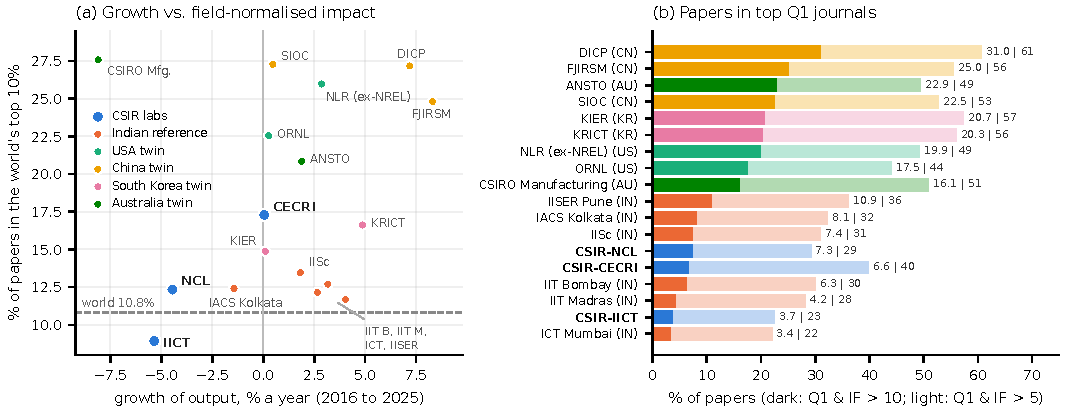
\includegraphics[width=\textwidth]{fig_global.pdf}
\caption{Global Benchmark, papers in the 31 benchmark subfields, 2016--2025. (a) Yearly growth against the share of papers in the world's top 10\% for their subfield, type and year (OpenAlex; the world's own share is 10.83\%). (b) Share of papers in Q1 journals with IF\,$>$\,10 (dark; value first) and IF\,$>$\,5 (light; value second), same SCImago rule as Table~1. Country codes: IN India, US, CN, KR, AU.}
\end{figure*}

\obs{Shrinking while the peers grow.} The labs' output changed by -4.5\% (NCL), -5.3\% (IICT) and 0.1\% (CECRI) a year, against 1.9\% for the twins (median) and 2.9\% for the Indian reference group; DICP and FJIRSM grew 7.2\% and 8.3\%.

\obs{Half the field-normalised impact.} The share of papers in the world's top 10\% is 8.9\% (IICT), 12.3\% (NCL) and 17.3\% (CECRI), against 10.83\% for the world, 12.3\% for the Indian reference group and 24.8\% for the twins (median): at home the labs are level with India's best, abroad they are at half the level (Fig.~3a).

\obs{The higher the bar, the wider the gap.} In plain Q1 share the twins are 1.2$\times$ ahead (median 78.3\% vs 64.7\%), with IF\,$>$\,5 1.8$\times$ (52.8\% vs 29.2\%), and with IF\,$>$\,10 3.1$\times$ (20.7\% vs 6.6\%; twins 16.1--31.0\%, labs 3.7--7.3\%, DICP 31.0\%). The Indian reference group sits with the labs (6.9\%). The labs' journal shares computed this way agree with the curated dataset (Table~1) within 3 points.

\begin{table}[t]
\centering\footnotesize\setlength{\tabcolsep}{2.4pt}
\caption{Each lab against its own foreign twins: lab value / twins' median (papers in the benchmark subfields, 2016--2025).}\label{tab:twins}
\begin{tabular}{@{}lcrrrrr@{}}
\toprule
Lab & Twins & Growth & Top 10\% & Q1\,\&\,IF$>$5 & Q1\,\&\,IF$>$10 & Intl. \\
 & & (\%/yr) & (\%) & (\%) & (\%) & (\%) \\
\midrule
NCL & 4 & -4.5 / +2.6 & 12.3 / 24.9 & 29.2 / 53.5 & 7.3 / 18.9 & 18.6 / 31.1 \\
\multicolumn{7}{@{}l}{\scriptsize\color{muted} twins: ORNL, DICP, KRICT, CSIRO Mfg.} \\[1pt]
IICT & 1 & -5.3 / +0.5 & 8.9 / 27.3 & 22.5 / 52.8 & 3.7 / 22.5 & 22.3 / 19.5 \\
\multicolumn{7}{@{}l}{\scriptsize\color{muted} twins: SIOC} \\[1pt]
CECRI & 4 & +0.1 / +2.4 & 17.3 / 22.8 & 39.9 / 52.5 & 6.6 / 21.8 & 31.1 / 25.8 \\
\multicolumn{7}{@{}l}{\scriptsize\color{muted} twins: NLR, FJIRSM, KIER, ANSTO} \\[1pt]
\bottomrule
\end{tabular}
\end{table}

\obs{Each lab, against its own twins.} The comparison holds lab by lab (Table~\ref{tab:twins}): every lab trails its own twins on growth, field-normalised impact and top-journal share. CECRI comes closest on impact, and IICT is furthest from its single twin, SIOC. Only in international co-authorship are IICT and CECRI ahead of their twins.

\obs{Who learns from whom.} The labs co-authored only 49 papers with the nine foreign twins and other foreign peers (8 with the twins themselves) against 682 with the six Indian institutes. Citations run inwards (Fig.~4a): the peers' 2016--2026 papers cite the labs 2,946 times while the labs cite 4,461 of theirs (exchange ratio 0.66; USA 0.40). At home the direction reverses: the Indian institutes' ratio is 1.38, and fifteen Indian universities draw on the labs more than the labs draw on them (IISc and IITs 1.63, state universities 2.00); two independent counts of these flows agree within 4.4\%.

\begin{figure}[t]
\centering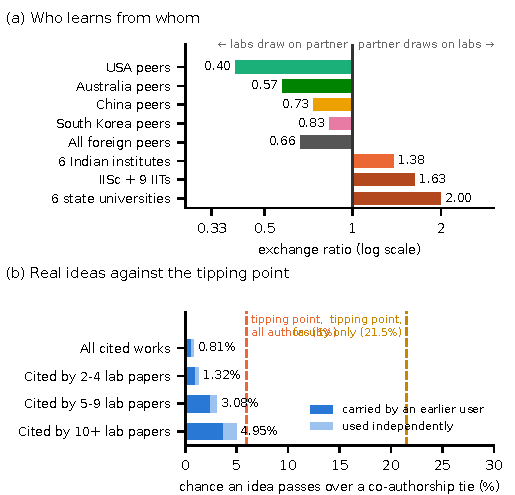
\includegraphics[width=\columnwidth]{fig_flows.pdf}
\caption{(a) Exchange ratio = partner papers citing the labs $\div$ partner papers the labs cite (2016--2026 papers, joint papers left out); below 1 the labs draw on the partner, above 1 the partner draws on the labs. (b) Share of (co-author tie, cited work) pairs in which the co-author later cites the work, from the labs' own papers, by how widely the work is reused; dashed: tipping points measured on the same networks (Section~5).}
\end{figure}

\section{How ideas spread through the labs}
\begin{table*}[t]
\centering\footnotesize\renewcommand{\arraystretch}{1.18}
\caption{Eight findings shown on the dashboard's main page (one script and one output file each; method notes on the dashboard).}\label{tab:findings}
\begin{tabular}{@{}>{\raggedright}p{2.35cm}>{\raggedright}p{9.0cm}>{\raggedright\arraybackslash}p{5.8cm}@{}}
\toprule
Finding & What we measured & What it means \\
\midrule
\textbf{Friendship paradox}\newline{\color{muted}\scriptsize Network} & 93.4\% of the 7,678 researchers have fewer co-authors than their co-authors (mean 9.0 vs 32.1); only 43.0\% of faculty do. & Hub and spoke: students and project staff reach the cluster through a few group leaders, who are the hubs. \\
\textbf{No rich club}\newline{\color{muted}\scriptsize Network} & The best-connected 1\% (81 researchers, 47 of them faculty) are less linked to each other than in randomised networks ($\rho_{norm} = 0.73$, 20 nulls). & No elite core: each leader runs a separate group, matching the separate communities of Section~3. \\
\textbf{Fragility}\newline{\color{muted}\scriptsize Network} & Removing the 886 highest-betweenness researchers (11.5\%) halves the largest component; random removal needs 3,325. Removing 675 of them separates the three labs' faculty. & Robust to random loss, fragile to the loss of a few bridges, who are worth protecting. \\
\textbf{Price's law}\newline{\color{muted}\scriptsize Productivity} & $\sqrt{N} = 18$ of 306 scientists write 36.9\% of faculty papers (the law predicts 50\%); the top 10\% write 49.1\%. Gini 0.61 (papers), 0.73 (citations). & Output is concentrated, impact more so: a few groups collect most of the citations. \\
\textbf{Q1 vs. impact}\newline{\color{muted}\scriptsize Journals} & 88.7\% of the cluster's top-10\% most-cited papers are in Q1 journals, yet only 14.0\% of Q1 papers reach the top 10\% (Q2--Q3: 3.5\%; 10,171 papers). & Q1 is close to necessary but far from sufficient, so the benchmark also uses field-normalised citations. \\
\textbf{Hidden gems}\newline{\color{muted}\scriptsize Citations} & In-cluster PageRank and global citations correlate only moderately (Spearman $\rho = 0.41$, 7,605 papers); 45 papers are in the top 5\% inside the cluster but below the median worldwide. & Some papers matter more to the labs' own later work than their citation counts show. \\
\textbf{COVID shock}\newline{\color{muted}\scriptsize Trends} & Output fell 8.6\% from 2019 to 2020 (1,320 $\to$ 1,207), but had been falling 8.6\% a year before; against that trend 2020 was 2.2\% and 2021 13.9\% above. Topic shift: JSD ratio 1.04. & No COVID-specific dip: the decline predates the pandemic, and the research mix barely changed. \\
\textbf{Brain circulation}\newline{\color{muted}\scriptsize Careers} & 17.0\% of 265 classifiable scientists trained in India, worked abroad and returned (25 of 45 in the USA). Their citations do not differ from peers of similar career age (+9\%, $p = 0.58$); 20.5\% vs 16.7\% of papers have a foreign co-author. & Time abroad shows up in foreign links, not in citations (classification awaiting manual validation). \\
\bottomrule
\end{tabular}
\end{table*}

\textbf{Model.} An idea (a method or reagent) spreads over the co-authorship network (SI dynamics, Monte Carlo and the NIMFA mean-field equations; bond percolation for tipping points). It reaches half of all 7,678 authors in 9 steps but half of the faculty-only network in 12; without students the tipping point is 3.6$\times$ higher (0.215 vs 0.06). Because co-authors form tight triangles (clustering 0.70), the measured tipping point is 1.54--2.32$\times$ the textbook value $\langle k\rangle/(\langle k^2\rangle-\langle k\rangle)$ in all networks. When transmission depends on topic overlap, ideas stay in their field (76.6\% of chemists adopt, 2.5\% outside). The mean-field equations never under-predict the simulation (28 runs) and rank the best seeds the same way ($\rho \ge$ 0.91).

\textbf{Tested on real citations.} Each of the 511,832 works the labs cite is an idea; a person adopts it with their first lab paper citing it (752,074 citations). Over a co-authorship tie an idea is passed on \textbf{0.81\%} of the time, 4.95\% for the most reused ideas: below the full network's tipping point (6\%; Fig.~4b), so most ideas die after one paper (79\% of cited works are used once). A student's tie passes ideas 2.7$\times$ as often as a faculty member's (1.51\% vs 0.56\%), though faculty have 35 co-authors against 5.6. Ideas travel with people: in 78\% of pass-ons an earlier user is an author of the new paper; one informed co-author barely changes a researcher's own use (1.17$\times$), three or more do (3.5$\times$). Only 1.4\% of ties cross labs, and a foreign twin's paper reaches a second lab through a person in 3.8\% of cases (the labs' own papers 22.8\%): together with Section~4, knowledge from abroad reaches each lab separately, by reading. All 15 claims of this study pass automatic checks (15/15).

\section{Further findings on the dashboard}
Beyond the two lead studies, the dashboard's main page carries eight focused findings, each computed by its own script with its method on the page; Table~\ref{tab:findings} gives what was measured and how to read it. Together they sharpen the picture above: a hub-and-spoke cluster held together by a few bridges, output and impact concentrated in a few groups, journal tier a weak proxy for a paper's use, and a decline that predates the pandemic.



\section{Validation and limitations}
Recall was boosted with raw-affiliation and roster searches, split author profiles joined and duplicates removed; peer rules and exclusions are stored with reasons, and every number is produced by tested code with fixed seeds. Limits: OpenAlex affiliations contain errors; faculty are today's rosters; IF is SCImago's two-year cites per document, not Clarivate's JIF, and SJR quartiles may differ from JCR; citations are a proxy for influence, not quality or patents; 2026 is a partial year.

\section{Conclusion}
The three laboratories are strong national performers: level with India's best institutes on field-normalised impact, a net source of knowledge for Indian universities, and moving their papers into higher-impact journals. Measured against government institutes abroad that do the same science, however, they publish less, are shrinking while the peers grow, and trail most at the very top (Q1 with IF\,$>$\,10), while hardly working with those peers or with each other. Closer collaboration across the three labs and with their foreign twins is the clearest lever the data points to.

\textbf{What the data points to.}
\begin{itemize}
\item \textbf{Connect the islands.} Only 0.8\% of co-authorship links cross labs, while 19.7\% of scientists' citations already do: the shared interest exists, the joint work does not.
\item \textbf{Work with the twins, not only read them.} The labs cite 4,461 of their foreign peers' papers but co-authored 49; ideas in these labs travel with people (78\% of real pass-ons), so joint papers are the channel that moves knowledge.
\item \textbf{Protect the bridges.} Removing 11.5\% of researchers, the best-connected bridges, halves the network; shared facilities such as crystallography already join groups that otherwise do not meet.
\item \textbf{Aim at the top band.} The gap to the twins is widest for Q1 journals with IF\,$>$\,10 (3.1$\times$), and the labs' share there is rising (1.8\% $\to$ 8.5\%).
\end{itemize}

\textbf{Data package.} The submission contains the dataset (\texttt{group24\_data.csv}, 14 required columns, and an extended version), the citation, co-authorship and Indian-connection networks, every table behind this report, the Global Benchmark's rules, exclusions, peer list and raw counts, the idea-spreading outputs with their checks, and an offline copy of the dashboard.

\end{document}
